% % % % % % % % % % % % % % % % % % % % % % % % % % % % % % % % % % % % % % % % % % % %
%                                                                                     %
% Short Sectioned Assignment LaTeX Template Version 1.0 (5/5/12)                      %
% This template has been downloaded from: http://www.LaTeXTemplates.com               %
%                                                                                     %
% Original author:  Frits Wenneker (http://www.howtotex.com)                          %
%                                                                                     %
% Modified by: Fco Javier Sueza Rodríguez (fcosueza@disroot.org)                      %
%                                                                                     %
% Changes:                                                                            %
%	    - Custom Chapters, Sections and Subsections (titlesec package)                %
%           - Document type scrbook (oneside)                                         %
%           - Use babel-lang-spanish package and marvosym                             %
%           - Use hyperref, enumitem, tcolorbox and glossaries packages               %
%           - Use Time New Roman (mathptmx), Helvetic and Courier fonts               %
%                                                                                     %
% License: CC BY-NC-SA 3.0 (http://creativecommons.org/licenses/by-nc-sa/3.0/)        %
%                                                                                     %
% % % % % % % % % % % % % % % % % % % % % % % % % % % % % % % % % % % % % % % % % % % %

%-----------------------------------------------%
%	              Packages                  %
%-----------------------------------------------%

\documentclass[paper=a4, fontsize=11pt, oneside]{scrbook}

% ---- Text Input/Output ----- %

\usepackage[T1]{fontenc}
\usepackage[utf8]{inputenc}
\usepackage{mathptmx}
\usepackage[scaled=.92]{helvet}
\usepackage{courier}
\usepackage[indent=12pt]{parskip}

\usepackage{geometry}
\geometry{verbose,tmargin=3cm,bmargin=3cm,lmargin=2.6cm,rmargin=2.6cm}

% ---- Language ----- %

\usepackage[spanish]{babel}
\usepackage{marvosym}

% ---- Another packages ---- %

\usepackage{amsmath,amsfonts,amsthm}
\usepackage{graphics,graphicx}
\usepackage{titlesec}
\usepackage{fancyhdr}
\usepackage{tcolorbox}
\usepackage{hyperref}
\usepackage{enumitem}
\usepackage[automake]{glossaries}

%--------------------------------------------------------------------%
%                      Customizing Document                          %
%--------------------------------------------------------------------%


% ----------- Custom Chapters, Sections and Subsections -------------- %

\titleformat{\chapter}[display]
			{\bfseries\Huge}
			{Tema \ \thechapter} {0.5ex}
			{\vspace{1ex}\centering}

\titleformat{\section}[hang]
			{\bfseries\Large}
			{\thesection}{0.5em}{}

\titleformat{\subsection}[hang]
			{\bfseries\large}
			{\thesubsection}{0.5em}{}

\titleformat{\subsubsection}[hang]
			{\bfseries\large}
			{\thesubsubsection}{0.5em}{}

\hypersetup{
    colorlinks=true,
    linkcolor=black,
    urlcolor=magenta
}

% ------------------- Custom heaaders and footers ------------------- %

\pagestyle{fancyplain}

\fancyhead[]{}
\fancyfoot[L]{}
\fancyfoot[C]{}
\fancyfoot[R]{\thepage}

\renewcommand{\headrulewidth}{0pt} % Remove header underlines
\renewcommand{\footrulewidth}{0pt} % Remove footer underlines

\setlength{\headheight}{13.6pt} % Customize the height of the header

% --------- Numbering equations, figures and tables ----------------- %

\numberwithin{equation}{section} % Number equations within sections
\numberwithin{figure}{section} % Number figures within sections
\numberwithin{table}{section} % Number tables within sections

% ------------------------ New Commands ----------------------------- %

\newcommand{\horrule}[1]{\rule{\linewidth}{#1}} % Create horizontal rule command


%----------------------------------------------------------------------------------------
%	TÍTULO Y DATOS DEL ALUMNO
%----------------------------------------------------------------------------------------

\title{
\normalfont \normalsize
\textsc{{\bfseries Curso 2022-2023} \\ Ciclo Superior de Desarrollo de Aplicaciones Web \\ IES Aguadulce} \\ [25pt]
\horrule{0.5pt} \\[0.4cm]
\huge Bases de Datos \\
\horrule{0.5pt} \\[0.4cm]
}

\author{Francisco Javier Sueza Rodríguez}
\date{\normalsize\today}

%----------------------------------------------------------------------------------------
%                                     DOCUMENTO
%----------------------------------------------------------------------------------------
\makeglossaries
\loadglsentries{glossary.tex}

\begin{document}

\maketitle

\newpage

\tableofcontents

\listoffigures

%\listoftables

\newpage

\chapter{Almacenamiento de la Información}
En este primer tema, vamos a estudiar los conceptos básicos sobre el almacenamiento de la información, así como de las bases de datos y los SGBD (Sistemas de Gestión de Bases de Datos), pero en primer lugar, vamos a hacer una introducción más detallada sobre que consideramos información y el contenido de este módulo.

\section{Introducción}
Si pensamos cualquier en cualquier aspecto de nuestra vida cotidiana, o si analizamos la mayoría de ámbitos de actividad, nos encontramos que la utilización de bases de datos esta ampliamente extendida. Estás, y los datos contenidos en ellas, serán imprescindibles para llevar a cabo multitud de acciones.

Algunas de las situaciones en las que es necesario el uso de bases de datos son las siguientes:

\begin{itemize}
    \item Cuando seleccionamos un canal de la TDT.
    \item Al utilizar la agenda del móvil para realizar una llamada telefónica.
    \item Cuando utilizamos un cajero automático.
    \item Cuando acudimos a la consulta del médico.
    \item Al inscribirnos en un curso, plataforma online, etc...
    \item Si utilizas el GPS.
    \item Cuando reservamos unas localidades en un evento deportivo.
    \item Cuando consultamos cualquier información en internet.
    \item Al solicitar un certificado de un organismo oficial.
\end{itemize}

Como vemos, el gran volumen de datos que manejamos y sus innumerables posibilidades hacen necesaria la existencia de técnicos perfectamente formados y capaces de trabajar con ellos.

Este módulo profesional se centra, precisamente, en las \textbf{Bases de Datos} y su uso en el desarrollo de aplicaciones. En esta primera unidad, comenzaremos conociendo los primeros sistema basados en ficheros para el almacenamiento y gestión de la información.  Seguidamente, se desarrollarán los conceptos y definiciones básicas relacionados con las bases de datos, viendo también sus modelos y tipos. Más adelante conocer los sistemas gestores de bases de datos y finalmente, veremos las herramientas reales con las que llevar a caso dicha gestión.

\section{Los Ficheros de Información}
En esta sección vamos a hablar de los fichero de información, en que consiste, que tipos nos podemos encontrar, métodos de acceso y parámetros de utilización.

\subsection{¿Que es un Fichero?}
En la década de los setenta, los procesos básicos relacionados con una empresa se centraban en la contabilidad y facturación. Las necesidades de almacenamiento y gestión de la información podían satisfacerse con un número relativamente reducido de archivos de papel agrupados y ordenados, los típicos ficheros clásicos.

Con la primera informatización, se paso del papel al ordenador, pudiendo acceder a los datos de forma mucho más rápida. Los ordenadores adaptaron sus herramientas para que se asemejaran a las que los usuarios utilizaban manualmente, de forma que en informática también empezó a hablarse de ficheros, carpetas, formularios, etc...

La información que empezó a tratarse en los ordenadores debía ser almacenada para su posterior recuperación, consulta y procesamiento. El elemento que se creo para almacenar esta información fue el \textbf{fichero} o \textbf{archivo}.

Podemos definir un \textbf{fichero} como el \textbf{conjunto de información relacionada}, tratada como un todo y organizada de \textbf{forma estructurada}. Es una secuencia de  dígitos binarios que organiza información relacionada con el mismo aspecto.

Los fichero están formados por \textbf{registros lógicos} que contienen información relativa a un mismo elemento u objeto (por ejemplo, información de un usuario). A su vez, los registros están divididos en \textbf{campos} que tienen cada una de las informaciones elementales que forman un registro (por ejemplo, nombre de usuario, email,...).

Los datos están almacenados de forma que se pueda añadir, suprimir, actualizar y consultar, individualmente, en cualquier momento.

Como los ficheros suelen ser muy grandes, solo se puede llevar parte de ellos a la memoria principal para procesarlos. La cantidad de información que es transferida entre el soporte en el que se almacena el fichero y la memoria del ordenador, en solo una operación de lectura/escritura, se llama \textbf{registro físico} o  \textbf{bloque}.

Normalmente en cada operación de lectura/escritura se transfieren varios registros de un fichero, es decir, un bloque suele contener varios registros lógicos. Al número de registros que entran en un bloque se le llama \textbf{factor de blocaje}, y a la operación de agrupar varios registros en un mismo bloque se conoce como \textbf{bloque de registros}.

\subsection{Tipos de Ficheros}
Según la función que vaya a desempeñar un fichero, estos pueden ser clasificados de varias maneras:

\begin{enumerate}[label=(\alph*)]
    \item \textbf{Ficheros Permanentes}: contiene información relevante para una aplicación. Es decir, los datos necesarios para el funcionamiento de ésta. Tiene un período de permanencia en el sistema amplio. Se subdividen en:
    \begin{itemize}
        \item \textbf{Ficheros Maestros}: contiene el estado actual de los datos que pueden modificarse desde la aplicación. Es la parte central de aplicación, su núcleo.
        \item \textbf{Ficheros Constantes}: son aquellos que incluyen datos fijos de la aplicación. No suelen ser modificados y se accede a ellos para la realización de consultar.
        \item \textbf{Ficheros Históricos}: contiene datos que fueron considerados como actuales en un período o situación anterior. Se utilizan para la reconstrucción de situaciones o estados concretos.
    \end{itemize}

    \item \textbf{Ficheros Temporales}: se utilizan para almacenar datos que son útiles para un parte de la aplicación. Son generados a partir de datos de ficheros permanentes y tienen un período corto de existencia. Estos pueden ser:
    \begin{itemize}
        \item \textbf{Ficheros Intermedios}: almacenan resultados de una aplicación que serán usados por otra.
        \item \textbf{Ficheros de Maniobras}: almacenan datos de una aplicación que no pueden ser mantenidos en memoria por falta de espacio.
        \item \textbf{Ficheros de Resultados}: almacenan datos que van a ser transferidos a un dispositivo de salida.
    \end{itemize}
\end{enumerate}

En la siguiente figura podemos ver un esquema con esta clasificación.

\begin{figure}[ht]
    \centering
    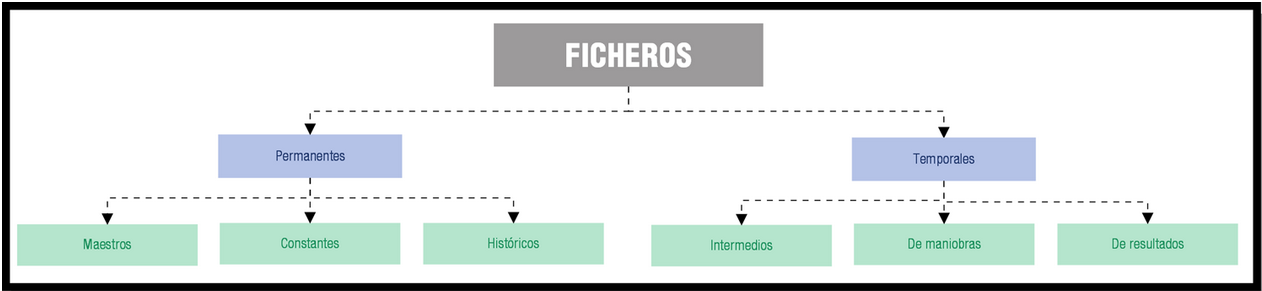
\includegraphics[scale=0.35]{ficheros-tipos.png}
    \caption{Clasificación de ficheros según su función}
\end{figure}

\subsection{Los Soportes de la Información}
Los ficheros se almacenan en soportes de información manejados por periféricos del ordenador, que permiten leer y grabar datos en el soporte. Los soportes más utilizados son las \textbf{cintas magnéticas} y los \textbf{discos} (magnéticos, ópticos o magneto-ópticos).

Al principio se usaban tambores de cinta magnética, similares en tamaño a un disco de vinilo, funcionaban de manera similar a los antiguos casetes, pero al tener un tamaño mucho más grande permitían almacenar mucha mas información, permitiendo el acceso a esta de forma secuencia.

Posteriormente los medios de almacenamiento fueron evolucionando a la par que el hardware, en concreto con la aparición de los disquetes y el disco duro. Estos dispositivos ya permitían el acceso aleatorio a los datos.

Por lo tanto, podemos distinguir dos tipos de dispositivos de almacenamiento de datos:

\begin{itemize}
    \item \textbf{Soportes de Acceso Directo a Datos}: son los más empleados y el acceso a datos se hacer de forma directa, pudiendo colocarlos en la posición que más nos interese.
    \item \textbf{Soporte de Acceso Secuencial}: se suele usar en copias de seguridad y si deseamos leer un dato que esta a mitad de la cinta, tendremos que leer todo lo que hay hasta llegar a esa posición.
\end{itemize}

Si quieres aprender más sobre las características de cintas y discos, puedes consultar los enlaces siguientes:

\begin{itemize}
    \item \href{https://es.wikipedia.org/wiki/Cinta_magn\%C3\%A9tica_de_almacenamiento_de_datos}{Cintas magnéticas de almacenamiento de datos}
    \item \href{https://es.wikipedia.org/wiki/Disco_magn\%C3\%A9tico}{Discos magnéticos} y \href{https://es.wikipedia.org/wiki/Disco_\%C3\%B3ptico}{Discos ópticos}
\end{itemize}

\subsection{Métodos de Acceso a Ficheros}
A medida que la tecnología ha ido evolucionando, el acceso a la información ha ido variando mucho. Los objetivos de fundamentales de estas variaciones son los siguientes:

\begin{itemize}
    \item Proporcionar acceso rápido a los registros.
    \item Conseguir economizar el almacenamiento.
    \item Facilitar la actualización de los registros.
    \item Permitir que la estructura refleje la organización real de la información.
\end{itemize}

Los ficheros se pueden clasificar según como se organiza en la memoria principal, o dicho de otra forma, los métodos de acceso al fichero, que podemos ver en la siguiente figura.

\begin{figure}[ht]
    \centering
    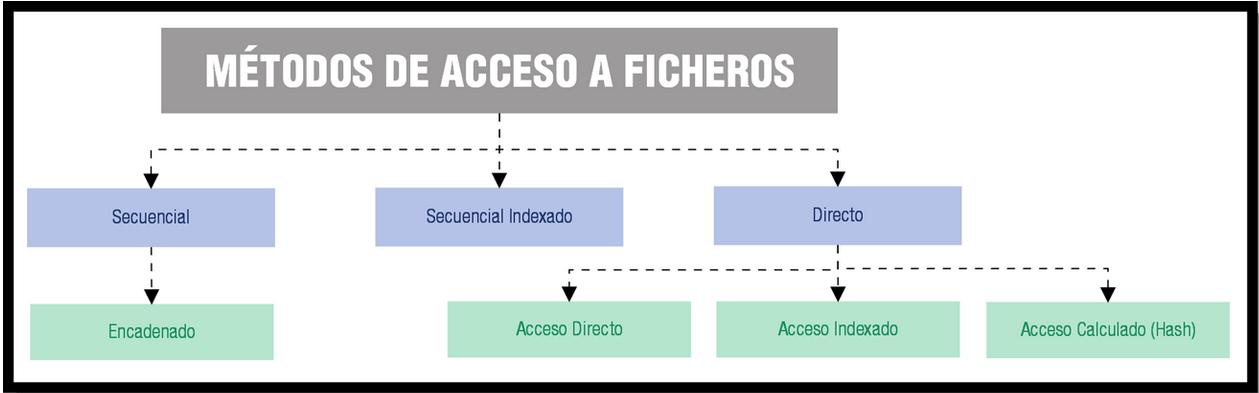
\includegraphics[scale=0.40]{ficheros-acceso.png}
    \caption{Tipos de ficheros por método de acceso}
\end{figure}

Las organizaciones secuencia, de acceso aleatorio o directo e indexado, son las mas comunes. En esta sección vamos a explicar las características de cada uno de los métodos de acceso a ficheros.

\subsubsection{Ficheros Secuenciales}
Un \textbf{fichero secuencial} se caracteriza porque sus registros están almacenados de forma continua, de forma que la única manera de acceder a él, es leyendo un registros detrás de otro hasta el final. En los ficheros secuenciales hay una marca que indica el final del fichero, suele denominarse \textbf{EOF} (End Of File). Así, para detectar el final de fichero solo es necesario encontrar esta marca.

Este tipo de fichero puede usar dispositivos de almacenamiento de acceso secuencial, como cintas magnéticas, aunque también se utilizan en los CD de audio y DVD de vídeo, en los que la música y las imágenes se almacenan en un espiral continua.

Los registros almacenados se identifican por medio de la información ubicada en uno de sus campos, que se denomina \textbf{clave} o \textbf{llave}. Si se ordena un archivo secuencial por su clave es más rápido realizar operaciones sobre el.

\begin{figure}[ht]
    \centering
    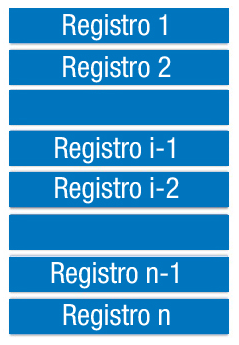
\includegraphics[scale=0.32]{fichero-secuencial.png}
    \caption{Estructura de un fichero secuencial}
\end{figure}

Algunas características de este tipo de ficheros son las siguientes:

\begin{itemize}
    \item La \textbf{lectura} siempre se realiza \textbf{hacia adelante}.
    \item Son ficheros \textbf{monousuario}, no permiten el acceso simultáneo de varios usuarios.
    \item Tiene una \textbf{estructura rígida de campos}. Todos los registros deben aparecer en orden, es decir, la posición de los campos en el registros siempre debe ser la misma.
    \item El \textbf{modo de apertura} del fichero, condiciona la lectura o escritura.
    \item \textbf{Aprovechan al máximo} el soporte de \textbf{almacenamiento}, no dejando huecos vacíos.
    \item Se pueden \textbf{grabar} en \textbf{cualquier tipo} de \textbf{soporte}, tanto secuenciales como direccionales.
    \item Todos los \textbf{lenguajes de programación} contiene instrucciones para \textbf{trabajar} con este tipo de ficheros.
    \item \textbf{No} se pueden \textbf{insertar registros} en los que están \textbf{ya grabados}.
\end{itemize}

\subsubsection{Ficheros de Acceso Directo}
En este tipo de archivos se puede acceder a un registro indicando la posición relativa del registros dentro del archivo, o a través de una \textbf{clave} que forma parte del registro como un \textbf{campo} más. Estos archivos deben almacenarse en dispositivos de memoria masiva con acceso directo como los discos magnéticos.

Cada uno de los registros se guarda en una posición física, que dependerá del espacio disponible en memoria masiva, por lo que la distribución es aleatoria dentro del soporte de almacenamiento. Para acceder a la posición física del registros se utiliza una posición o índice, de forma que no es necesario recorrer todo el fichero para encontrar un determinado registros.

 Esta \textbf{dirección física} se obtendrá tras la aplicación de una \textbf{transformación} específica a la \textbf{clave}. Según como sea esta transformación, existen tres modos de acceso diferente, como podemos ver en la siguiente figura.

\begin{figure}[ht]
     \centering
     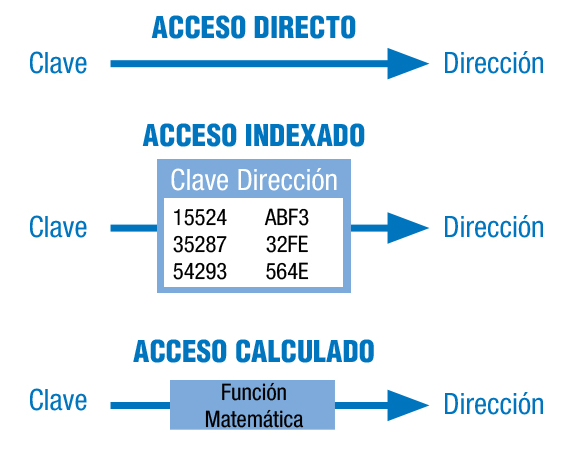
\includegraphics[scale=0.32]{fichero-accesodirecto.png}
     \caption{Modos de acceso a un registro en archivos de acceso directo}
 \end{figure}

El método más rápidos es el \textbf{acceso directo}, donde la clave coincide con la dirección física del registro, teniendo ésta que ser una posición valida dentro del rango de direcciones físicas.

La \textbf{medida de posicionamiento} básico del puntero en el fichero es el \textbf{byte}, dependiendo del tipo de codificación de caracteres que empleemos (\textbf{\gls{Unicode}}, \textbf{\gls{ANSI}}), se usarán 1 o 2 bytes por carácter respectivamente. Teniendo esto en cuenta, el puntero avanza de 1 en 1 o de 2 en 2 bytes para poder leer o escribir cada carácter.

Otras \textbf{características} de este tipo de ficheros son las siguientes:

\begin{itemize}
    \item \textbf{Posicionamiento inmediato}.
    \item \textbf{Registros} de \textbf{longitud fija}.
    \item \textbf{Apertura} del fichero en \textbf{modo mixto}, para lectura y escritura.
    \item Permiten \textbf{múltiples usuarios} al mismo tiempo.
    \item Los \textbf{registros se borran} colocando un cero en la posición que ocupan.
    \item Permiten la utilización de \textbf{algoritmos de compactación} de huecos.
    \item Los archivos se \textbf{crean} con un \textbf{tamaño definido}, es decir, con un máximo de registros definidos durante su creación.
    \item Esta organización solo es posible en \textbf{soportes direccionales}.
    \item Se \textbf{usan} cuando el \textbf{acceso a datos} de un registro se hace siempre empleando la \textbf{misma clave} y la \textbf{velocidad de acceso} al registro es lo que más importa.
    \item Permiten la \textbf{actualización de registros} en el mismo fichero, sin necesidad de copiarlo.
    \item Permiten realizar \textbf{procesos de actualización} en \textbf{tiempo real}.
\end{itemize}

\subsubsection{Ficheros Indexados}
Se basan en el uso de \textbf{indices}, que permiten el acceso a un registros sin tener leer el fichero entero. Estos indices son similares a los de los libros, si nos interesa leer un capítulo podemos recurrir al indice donde se nos dice en que página comienza y acaba dicho capítulo.

Por lo tanto, deberá existir una \textbf{zona de registros} en los que se encuentren los datos del archivo y una \textbf{zona de índices}, que contiene la tabla con las claves de los registros y las posiciones donde se encuentran. La tabla de índices esta ordenada por campos clave.

La tabla de índices será cargada en la memoria principal para realizar en ella la búsqueda de la fila correspondiente a la clave del registros a encontrar, proporcionando así la dirección donde se encuentra el registro. Una vez localizada la dirección, solo es necesario acceder el dispositivo de almacenamiento y colocarlos en la dirección indicada.

\begin{figure}[ht]
    \centering
    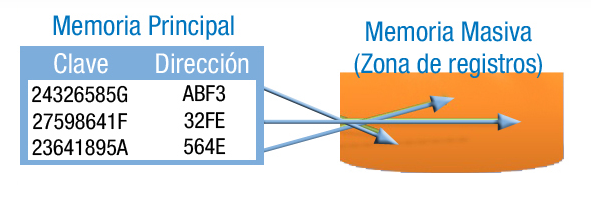
\includegraphics[scale=0.50]{fichero-indexado.png}
    \caption{Ficheros indexados}
\end{figure}

Las características mas relevantes de los ficheros indexados son las siguientes:
\begin{itemize}
    \item El diseño de registros tiene que tener un campo o campos, que permita identificar cada registro de forma única, es decir, no puede haber 2 registros que tengan la misma información en él. A este campo se le llama \textbf{campo clave} y es el que va a servir de índice. Un mismo fichero puede tener varios campos clave, pero al menos uno de ellos \textbf{no puede tener valores duplicados} y se llama \textbf{clave principal}. A las restantes se les llama \textbf{claves alternativas}.
    \item Permite usar el modo de \textbf{acceso secuencial} y el modo de \textbf{acceso directo} para leer la información que guardan sus registros.
    \item Para acceder a estos ficheros usando el modo de \textbf{acceso directo}, se hace conociendo el \textbf{contenido} del \textbf{campo clave} que queremos localizar. Con esta información el sistema operativo puede consultar el índice y conocer la posición dentro del fichero.
    \item Para acceder a este tipo de ficheros usando el m\textbf{modo secuencial}, los registros son \textbf{leídos} por el contenido del \textbf{campo clave}, independientemente del orden en el que fueron grabados, ya que el acceso se hace a través del índice, que para hacer más fácil la búsqueda de registros, permanece siempre ordenado por campos clave.
    \item Solamente puede \textbf{almacenarse} en un \textbf{medio direccionable}, ya que sino no podría usar el modo de acceso directo.
\end{itemize}

\subsubsection{Otros Tipos de Organización}
Además de los tipos de organización de ficheros que ya hemos visto, existen otros como los \textbf{ficheros secuenciales indexados} o los \textbf{ficheros de acceso calculado}, los cuales pasamos a describir a continuación.

\begin{enumerate}[label=(\alph*)]
    \item \textbf{Ficheros Secuenciales Indexados}:

    También llamados parcialmente indexados, al igual que los ficheros indexados existe una \textbf{zona de índices} y otra \textbf{zona de registros de datos}, pero esta última se encuentra \textbf{dividida} en \textbf{segmentos} ordenados.

    En la zona de índices, cada fila hace referencia a cada uno de los segmento. La clave corresponde al último registros del segmento y el índice al registro inicial. Una vez que se accede al primer registro del segmento, dentro de él se localiza (de forma secuencial) el registro buscado.

    Las principales características de este tipo de ficheros son:
    \begin{itemize}
        \item Permite el \textbf{acceso secuencial}. Esto es muy interesante cuando la tasa de accesos es alta. En el acceso secuencial ademas los registros se leen ordenados por el campo clave.
        \item Permite el \textbf{acceso directo a registros}. Realmente \textbf{emula} este tipo de acceso, empleando para ello las tablas de índices. Primero busca la clave en el área de índices y luego va a leer al área de datos en al dirección que indica la tabla.
        \item Se pueden \textbf{actualizar} los \textbf{registros} en el \textbf{mismo fichero}, sin necesidad de crear uno nuevo de copia en el proceso de actualización.
    \end{itemize}
\end{enumerate}

% Glossary

\glsaddall
\printglossaries

% Bibliography

\newpage
\addcontentsline{toc}{chapter}{Bibliografía}
\bibliography{citas}
\bibliographystyle{unsrt}

\end{document}